\chapter{Realisierung}\label{ch:realisierung}
In diesem Kapitel wird die Implementierung eines Templates zur Beantwortung der Forschungsfragen der Arbeit\footnote{Siehe Absatz \ref{sec:ziel}} beschrieben.
Dazu wird nach der im Kapitel \ref{ch:vorgehensweise} beschriebenen Reihenfolge der Arbeitsschritte vorgegangen.
Es ist noch einmal zu erwähnen, dass zunächst abzuwägen ist, welche Implementierungsvariante des \glqq IBM Cloud Provisioning and Management for z/OS\grqq besser geeignet ist: z/OSPT oder z/OSMF.
Die Provisionierung einer CICS-Instanz wird vorerst auf dem Testplex untersucht.
Danach wird in weiteren Schritten zuerst eine Db2 Datenbank und schließlich IBM MQ Queues dem Bereitstellungsprozess hinzugefügt.
Um einen Testablauf der DATEV-Rechnungsschreibung mit der so generierten Laufzeitumgebung durchführen zu können, muss das Template auch in der Entwicklungsstage verfügbar sein.
Ist dies sichergestellt wird der dadurch ermöglichte Bereitstellungsprozess anhand von drei Use-Cases aufgezeigt.
Es folgt ein Fazit zu dieser Implementierung.
Zuletzt folgt eine Bewertung der implementierten Provisionierungslösung durch die Stakeholder bei DATEV e.G. (Entwickler, Administration, Technologiestrategie).

\section{Vergleich zwischen z/OSPT und z/OSMF}
Bei beiden Varianten steht sowohl eine schnelle Provisionierung, als auch Deprovisionierung von Instanzen durch den Entwickler im Vordergrund.
Mittels Templates läuft beides automatisiert, verlässlich, und ohne manuelle Abstimmungen ab.
Die Bereitstellung einer Instanz ist wiederholbar, so kann die Instanz z.B. im Fehlerfall sicher neu erstellt werden und muss nicht langlebig gepflegt werden. 

Es folgt ein Vergleich der beiden Tools an Hand folgender Kriterien:
\begin{samepage}
\begin{itemize}
\item Schnittstelle
\item Verwaltung von Templates
\item Verwaltung von Instanzen bzw. Containern
\item Einsatz von Images
\end{itemize}
\end{samepage}

Aus der Tabelle \ref{tab:vglzosptzosmf} ergibt sich folgendes Fazit:\\
z/OSPT ist durch den Einsatz von Images deutlich flexibler bezüglich der Konfigurationsmöglichkeiten der Templates.
Jedoch ist die browserbasierende Schnittstelle von z/OSMF intuitiver als ein Kommandozeileninterface, dadurch fällt die Einarbeitung in automatisierte Bereitstellungsmechanismen leichter.
Hinzu kommt, dass innerhalb von z/OSPT für die Zuweisung von Domains und Tenants eine weitere externe Konfigurationsdatei gepflegt werden muss.

Ausschlaggebender Grund für das Nutzen von z/OSMF für die Beantwortung der Forschungsfragen ist die browserbasierende Oberfläche.
Die damit ermittelten Forschungsergebnisse sind aber auch als Basis für eine Bewertung von z/OSPT nutzbar.
\begin{table}
\centering
\begin{tabularx}{\textwidth}{r|X|X}
Kriterium & z/OSPT & z/OSMF\\
\hline
Schnittstelle & Kommandozeile & browserbasierende Oberfläche\\
\hline
Verwaltung von Templates & Zuweisung von Domains und Tenants nicht intuitiv & Alle Arbeitsschritte intuitiv\\
\hline
Verwaltung von Instanzen bzw. Container &  möglich & möglich\\
\hline
Einsatz von Images & Ja & Nein\\
\end{tabularx}
\caption{Vergleich zwischen z/OSPT und z/OSMF}
\label{tab:vglzosptzosmf}
\end{table}

\section{Testplex}
Der Zugriff auf Ressourcen und Tools bei DATEV e.G. wird über ein Rechtekonzept über RACF verwaltet. 
Um die Forschungsfragen beantworten zu können, mussten vor Beginn der eigentlichen Untersuchung zunächst alle benötigten Rechte beantragt werden.
Hierzu zählen unter anderem die Rechte für die Nutzung des Testplexes, die Nutzung von z/OSMF und z/OSPT und die Rechte für die Templateverwaltung innerhalb von z/OSMF. 
Beispielsweise benötigt \glqq IBM Cloud Provisioning and Management for z/OS\grqq{} lesenden Zugriff auf den Speicherpfad der Template Dateien.
Auf dem Testplex ist es  möglich, die Rechte für das Erstellen der CICS Dateien, das Starten einer CICS Instanz und die Administration von Db2 und IBM MQ einer persönlichen UserID zu geben, was in der Entwicklungsstage nicht ohne weiteres umsetzbar ist. 

Schließlich konnte, wie in Kapitel \ref{ch:vorgehensweise} beschrieben, mit dem ersten Versuch, das bei der Installation von z/OSMF mitgelieferte \glqq cics\_getting\_started\grqq{} Template zu provisionieren, begonnen werden.
Ziel war es, mit dem Tool vertraut zu werden und die grundsätzliche Lauffähigkeit zu prüfen.

\subsection{\glqq cics\_getting\_started \grqq-Template}\label{ssec:cgs}
Da es sich, wie in Kapitel \ref{ch:vorgehensweise} beschrieben, um ein mitgeliefertes Template handelt, sind alle benötigten Workflowdefinitionsfiles und Template Dateien vorhanden.
Wie in Absatz \ref{sssec:zosmf} aufgezeigt, muss das Template in die Software Services von z/OSMF aufgenommen werden.
Hierzu müssen die Template-und Workflow-Dateien in einem Unix Dateisystem auf dem Großrechner abgelegt sein. 
Nach dem Aufnehmen werden dem Template noch eine Domain und ein Tenant zugewiesen.\footnote{Siehe \ref{sec:tool}}

Folgende Variablen sind in dem Variableinputfile nur mit Platzhaltern versehen und müssen für eine erfolgreiche Provisionierung ersetzt werden:
\begin{table}[h]
\centering
\begin{tabularx}{\textwidth}{X|X}
Variablenname & Kurzbeschreibung \\
\hline
DFH\_REGION\_APPLID & Applikations ID der zu provisionierenden CICS-Instance. \\
\hline
DFH\_REGION\_HLQ & High-level qualifier für die CICS Dateien.\\
\hline
DFH\_STC\_ID & User ID mit dem die CICS-Instanz startet. \\
\hline
DFH\_REGION\_VTAMNODE & Name des VTAM Knotens, wenn die CICS-Instanz hochfährt. \\
\hline
DFH\_CICS\_USSHOME & Homeverzeichnes des Unix System Services \\
\hline
DFH\_CICS\_HLQ & High-level qualifier von dem CICS Installationsort. \\
\end{tabularx}
\caption{Zu verändernde Variablen im \glqq cics\_getting\_started \grqq-Template}
\label{tab:cgsvars}
\end{table}

Als nächster Schritt wurde ein Testlauf und somit ein erster Versuch, das Template zu provisionieren, durchgeführt.
Dabei kam es anfangs trotz Testplex-Umgebung zu Rechteproblemen, da die Anforderungen und Rahmenbedingungen der DATEV e.G. in dem standardisierten IBM Template natürlich nicht berücksichtigt waren.
Beispielsweise ist die Berechtigung für das Starten von Jobs von DATEV Vorgaben abhängig und CICS-Start-Mechanismen haben spezifische Anforderungen an die Eingabeparameter.
Nach den notwendigen Anpassungen wurde das \glqq cics\_getting\_started \grqq-Template provisioniert und die definierten Aktionen aus dem Actiondefinitionfile getestet.
Dabei wurde sich auf das Nutzen der z/OSMF Oberfläche fokussiert und nicht auf die eigentliche Funktionsfähigkeit der CICS-Instanz. 

\subsection{\glqq cics\_54\grqq-Template}
Wie in Kapitel \ref{ch:vorgehensweise} bereits beschrieben, ermöglicht das \glqq cics\_54\grqq-Template komplexere Konfigurationsmöglichkeiten.
Es mussten neben den in Tabelle \ref{tab:cgsvars} genannten Variablen noch folgende, in Tabelle \ref{tab:c54vars} genannte Variablen gesetzt werden.
Die Kurzbeschreibungen und die Beschreibungen aller weiteren Variablen, die im Standard Template vorhanden sind, sind unter \cite{.26.2.2020b} zu finden.

\begin{table}[h]
\centering
\begin{tabularx}{\textwidth}{X|X}
Variablenname & Kurzbeschreibung \\
\hline
DFH\_REGION\_SEC & Legt fest, ob für das CICS Sicherheit im Allgemeinen aktiviert ist. \\
\hline
DFH\_REGION\_SECPRFX & Wenn DFH\_REGION\_SEC gesetzt ist, legt den Namen Prefix bei Authentificationanfragen für Ressourcen fest. \\
\hline
DFH\_LE\_HLQ & High-level qualifier\footnote{Erste Zeichen eines Dateinamens, wird zum Filtern genutzt} für die Sprachumgebung\footnote{Grundeinstellungen der Programmiersprachen COBOL, PLI und C. Mitgelieferte IBM Grundmodule} \\
\hline
DFH\_REGION\_LOGSTREAM & Legt fest, wie die Log Dateien für die provisionierte CICS-Instanz erstellt werden sollen. \\
\hline
DFH\_REGION\_DFLTUSER & Default User ID für die CICS-Instanz. \\
\hline
DFH\_REGION\_MEMLIMIT & Dem CICS maximal zur Verfügung stehender Speicherplatz. \\
\hline
DFH\_ZOS\_PROCLIB & Datei auf dem Großrechner, die den Job enthält, der für das Erzeugen der CICS-Instanz zuständig ist. \\
\hline
DFH\_ZOS\_VSAM\_VOLUME & Speichersystem auf welchem die Dateien gespeichert werden sollen. Entscheidung kann auch an das System abgegeben werden. \\
\end{tabularx}
\caption{Zu verändernde Variablen im \glqq cics\_54\grqq-Template}
\label{tab:c54vars}
\end{table}
Es wurden die gleichen Änderungen bezüglich der DATEV Job Vorgaben und der spezifischen Anforderungen der CICS-Start-Mechanismen wie in Absatz \ref{ssec:cgs} durchgeführt.
Nach Aufnahme in z/OSMF konnte die Provisionierung und Deprovisionierung erfolgreich durchgeführt werden.
Dadurch wurden erste Erfahrungen mit z/OSMF und die grundsätzliche technische Funktionsweise in der echten DATEV e.G. Entwicklungsumgebung erprobt, was vor allem für die CICS-Administratoren einen wichtigen Schritt darstellte.
Dennoch handelt es sich erst einmal um eine IBM Standard CICS Instanz, die nicht mit einer DATEV e.G. spezifischen CICS Instanz zu vergleichen ist.

\subsubsection{DATEV e.G. spezifisches CICS Template}\label{sssec:datevcics}
Ziel dieses  Schritts war die Provisionierung einer funktionsfähigen DATEV e.G. spezifischen CICS Instanz. 
In der im letzten Schritt provisionierten Standard IBM CICS-Instanz sind z.B. keine DATEV e.G. internen Transaktionen verfügbar.
Dabei handelt es sich um interne Management-Transaktionen, mit denen z.B. Entwickler ihre fachlichen Transaktionen verwalten. 
Beispielhaft sei hier die Transaktion XMON zu erwähnen, ein DATEV proprietäres Auskunftssystem über CICS-Transaktionen, Programme, Dateien usw.
Dies ist auch in einer automatisiert provisionierten CICS-Instanz notwendig.

Um dieses Template an die DATEV Umgebung anzupassen und letztendlich eine \glqq DATEV CICS Instanz\grqq{} zu provisionieren, wurden folgende Schritte durchgeführt.

\begin{samepage}
\begin{itemize}
\item Analyse des bestehenden Templates und der darauffolgenden Überarbeitung 
\item Umgang und Anpassung der CSD Datei
\item Anpassung der Jobs und Skripte mit Schwerpunkt auf der \glqq createCICS.jcl\grqq-JCL-Datei\footnote{Quellcode siehe Anhang \ref{app:createcics}}.
\end{itemize}
\end{samepage}

Die Analyse ergab, dass das mitgelieferte \glqq cics\_54\grqq-Template mit insgesamt 76 verwendeten Dateien sehr komplex und umfangreich ist.
Es zählen alle Dateien, die direkt mit dem Template in Verbindung stehen.
Im Zentrum des Templates steht die Workflow Definitionsdatei \glqq provision.xml\grqq{} mit circa 583 Zeilen Code.
In dieser sind alle Steps, die bei einer Provisionierung durchgeführt werden, definiert.
Das Template beinhaltet nicht nur die Möglichkeit, CICS Instanzen mit unterschiedlichen Konfigurationen zu provisionieren, sondern auch, festzulegen, ob dies mit Skripten oder mit der REST-API geschieht.

Die Grundstruktur des \glqq cics\_54\grqq-Templates wurde beibehalten, allerdings wurden nach dem \glqq YAGNI\grqq-Prinzip\footnote{\glqq You aren't gonna need it\glqq-Prinzip} alle für eine DATEV e.G. spezifische CICS Instanz nicht benötigten Steps, die dazugehörigen Variablen und Dateien entfernt.
Wie in Tabelle \ref{tab:vglTemps} zu sehen ist, konnten dadurch circa die Hälfte der Dateien gelöscht werden und bei der provision.xml konnte ein Drittel an Quellcode eingespart werden.
Somit gewinnt das Template an Übersichtlichkeit und kann dadurch einfacher angepasst und gewartet werden.
Das überarbeitete Template dient dem weiteren Vorgehen als Grundlage.

\begin{table}[h]
\centering
\begin{tabularx}{\textwidth}{r|X|X}
& IBM Standard CICS Template & DATEV e.G. spezifisches Template \\
\hline
Verwendete Dateien & 76 & 36 \\
\hline
provision.xml & circa 583 Codezeilen & circa 199 Codezeilen. \\
\end{tabularx}
\caption{Vergleich der beiden Templates in Bezug auf deren Umfang}
\label{tab:vglTemps}
\end{table}

Wie in Absatz \ref{ssec:aktcics} beschrieben, benötigt eine CICS Instanz spezifische Dateien.
Die Namen dieser CICS Dateien wurden im dafür zuständigen Job an die DATEV e.G. internen Namenskonventionen angepasst.

Die nächste Voraussetzung für die Bereitstellung einer CICS Instanz ist das Erstellen einer CSD-Datei\footnote{Beschreibung siehe Absatz \ref{ssec:aktcics}}.
Folgende Entscheidung wurde in Zusammenarbeit mit dem CICS Administratorenteam getroffen.
Um Auswirkungen auf bereits im Einsatz befindliche Instanzen zu verhindern, wird die von den Kollegen gepflegte CSD-Datei bei jeder Provisionierung kopiert und mit bestimmten Namenskonventionen gespeichert.
So besitzt jede automatisch bereitgestellte CICS Instanz eine eigene CSD Datei.
Durch dieses Vorgehen wird zudem sichergestellt, dass bei jeder Provisionierung die aktuellste Version der CSD Datei verwendet wird.
Im Falle einer gemeinsamen CSD Datei für alle provisionierten Instanzen müssten Änderungen, wie beispielsweise die Verfügbarkeit einer neueren CICS Version, an einer weiteren Stelle angepasst werden.
Wird als Basis aber die aktuell schon verwaltete CSD Datei verwendet, genügt eine Neuprovisionierung des Templates um die Änderung auch für die provisionierten Instanzen zu übernehmen.
Neue Ressourcen, wie zum Beispiel eine Verbindung zu einem Db2 Subsystem, können so ohne Nebenwirkungen zu anderen CICS Instanzen in die CSD aufgenommen werden.
Ein weiterer Vorteil ist, dass bei der Deprovisionierung der CICS-Instanz diese Kopie der Standard Datei ohne Nebenwirkungen gelöscht werden kann.

Um dies umzusetzen, wurden zunächst zwei JCL Jobs geschrieben und in das entsprechende Workflowdefinitionfile eingebunden.
Einer für die Implementierung des Kopiervorgangs und einer zum Löschen dieser Kopie.
Für die Anpassung der CSD der zu provisionierenden Instanz ist ein weiterer Job, der \glqq InitAdditionalCSD.jcl\grqq-Job, notwendig.
Es mussten bestimmte Gruppen (Zeilen sieben, neun und zehn in Abbildung \ref{code:addCSD}) zu der CSD Liste der CICS Instanz hinzugefügt werden.
Dabei handelt es sich um Ressourcen, die jede DATEV e.G. CICS Instanz benötigt.
Die Reihenfolge ist relevant, da sie der Initialisierungsreihenfolge beim Startvorgang der CICS Instanz entspricht.
Diese beiden Jobs wurde jeweils als neuer Workflowdefinitionfile-Step in den z/OSMF Workflow eingebunden.

\begin{minipage}{\linewidth}
\lstinputlisting[caption={Hinzufügen weiterer CSD Gruppen zur Liste der provisionierten CICS-Instanz mittels des Jobs \glqq InitAdditionalCSD.jcl\grqq},captionpos=b,label={code:addCSD}]{listings/initaddCSDalt.jcl}
\end{minipage}

Der abschließende Schritt zur Bereitstellung einer CICS Instanz ist das Erzeugen des STC Jobs.
Die Definition bzw. das Script zur Erzeugung dieses Jobs ist in der \glqq createCICS.jcl\grqq-JCL-Datei zu finden.
Im \glqq cics\_54\grqq-Template beinhaltet diese ein Makro für die Validierung der SIT Parameter.
Zusätzlich werden alle aus der Datei für die Eingabevariablen benötigten Variablenwerte in temporäre Zwischenvariablen eingefügt.
Danach folgt die Definition des Jobs, diese setzt sich aus folgenden Hauptbestandteilen zusammen:

\begin{itemize}
\item Einbindung der benötigten Bibliotheken
\item Einbindung der zuvor angelegten CICS spezifischen Dateien
\item Definition der SIT Parameter
\end{itemize}

Für das Einbinden der benötigten Bibliotheken und der zuvor angelegten CICS spezifischen Dateien ist nur das Hinzufügen weiterer DD-Statements notwendig.

In Abbildung \ref{code:sitparams} ist zu sehen, dass es vor allem bei der Definition der SIT Parameter zu tief verschachtelten if-Bedingungen kommen kann.
Es handelt sich um den Code, der für das Einlesen der Variable  \glqq DFH\_REGION\_SITPARAMS\grqq{} aus der Eingabedatei zuständig ist.
In dieser Variable werden die SIT Parameter als Komma separierter String angegeben.
Für die Erzeugung eines DATEV e.G. spezifischen CICS wurde das ursprünglich in dem Template verwendete Makro für die Validierung von SIT Parametern beibehalten.
Alles danach wurde zunächst durch eine zur Verfügung gestellten DATEV e.G. Standard JCL, für die Erzeugung eines CICS, ersetzt.
Nach und nach wurde damit die für die DATEV e.G. spezifische CICS Provisionierung notwendige Logik, (siehe Abbildung \ref{code:sitparams}), hinzugefügt.
Damit wurde die vorher statische DATEV e.G. Standard JCL für das Erstellen von CICS Instanzen durch die Verwendung von Template  Variablen flexibilisiert.

\begin{minipage}{\linewidth}
\lstinputlisting[caption={Setzen der SIT Parameter durch Auslesen der \glqq DFH\_REGION\_SITPARAMS\grqq{} Variablen. (Zeile 379 bis 401 aus der \glqq createCICS.jcl\grqq-JCL-Datei, siehe Anhang \ref{app:createcics})},captionpos=b,label={code:sitparams},firstline=379, lastline=401]{listings/CreateCICS.jcl}
\end{minipage}

Es wurden nur die wirklich benötigten SIT Parameter aufgenommen.
Die anzunehmenden Werte wurden einzeln mit dem CICS Administratorenteam besprochen und festgelegt.
Es ist zu beachten, dass es im IBM Standard Template zwei Möglichkeiten gibt, diese Parameter zu setzen.
Für bestimmte SIT Parameter existiert eine Variable innerhalb des Templates.
Für alle anderen ist die Variable \glqq DFH\_REGION\_SITPARAMS\grqq{} vorgesehen.
In dieser Arbeit wurde hauptsächlich mit letzterer Variante gearbeitet.
Dadurch sind die SIT Parameter nur an einer Stelle im Template zu verwalten, beziehungsweise wird die Verwaltung  nicht auf zwei Arbeitsweisen verteilt.

Durch die beschriebene Vorgehensweise wurde erfolgreich die Provisionierung einer DATEV e.G. spezifischen CICS Instanz umgesetzt.
Getestet wurde die Nutzbarkeit der Instanz mit einem Anmeldevorgang an dieses CICS, wie in Abbildung \ref{fig:cicslogin} zu sehen ist.
Darüber hinaus wurde erfolgreich nachgewiesen, dass Standard Transaktionen der DATEV e.G.  in dieser Instanz funktionsfähig sind.
Die Deprovisionierung verlief nach Plan.

\begin{figure}[h]
	\centering
	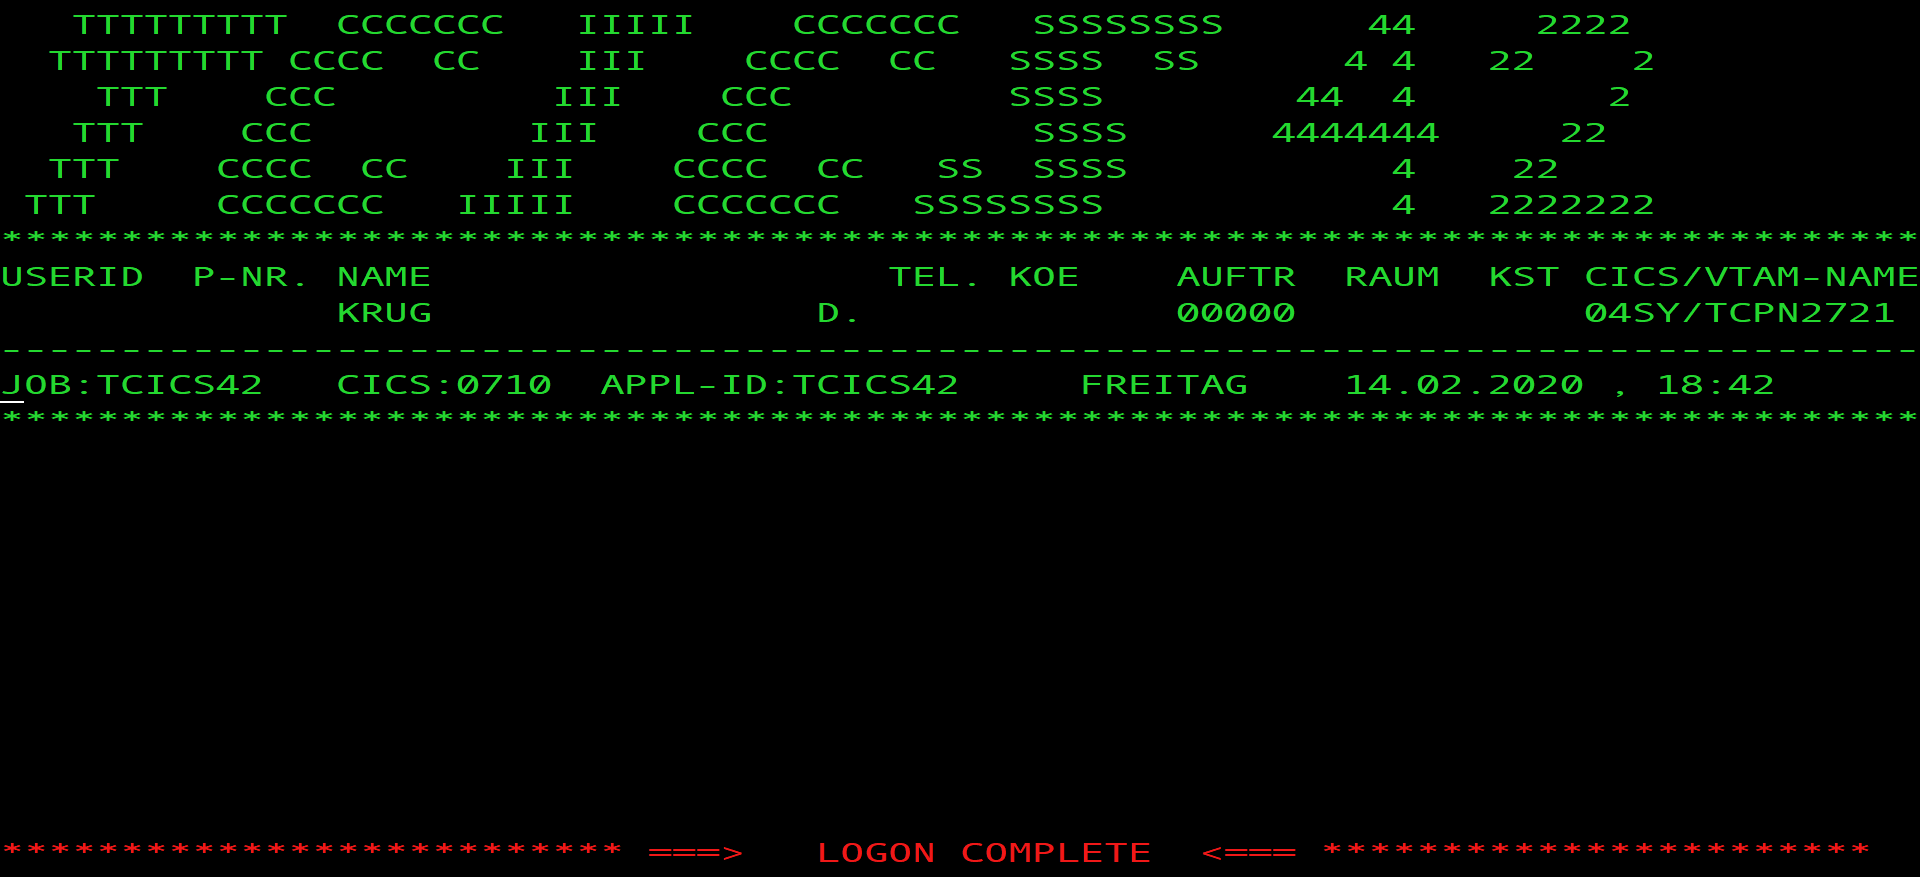
\includegraphics[width=\textwidth]{figures/logonscreen.PNG}
	\caption{Login Bildschirm der provisionierten DATEV spezifischen CICS-Instanz}
	\label{fig:cicslogin}
\end{figure}

\subsubsection{Bereitstellung Db2}\label{sssec:db2tpl}
In diesem Absatz wird die Provisionierung einer Db2 Datenbank Instanz beschrieben.
In der Systemumgebung Testplex bedeutet dies die Provisionierung der Datenbank Instanz ohne Tabellen und Daten.

Für die Erstellung einer Db2 Datenbank existiert innerhalb der DATEV e.G. bereits ein \glqq Self Service\grqq.
Dieser stellt für die Provisionierung einer Db2 Datenbank auch eine REST-API zur Verfügung.
Wie im Absatz \ref{sec:tool} beschrieben, ist es möglich, innerhalb eines Workflow Steps einen REST-Request abzusenden.
Der Code ist in Abbildung \ref{app:db2prov} im Anhang zu finden.
So muss im Body des Requests unter anderem der Datenbankname und eine UserID übergeben werden.
Der Code für das Löschen der Datenbank sieht ähnlich aus, nur handelt es sich in diesem Fall um einen DELETE-Request.
Die zwei notwendigen Steps wurden erzeugt und in den Workflow eingebunden.

Die API ist nur dazu fähig, Datenbanken auf dem DB0C Sandbox Datenbankmanagementsystem\footnote{Siehe Absatz \ref{sssec:db2}} zu erzeugen.
Um die Datenbank aus der CICS-Instanz heraus nutzen zu können, muss dem CICS dieses Datenbanksystem mitgeteilt werden.
Hierfür ist, wie in Abbildung \ref{code:addCSD} in Zeile acht bereits zu sehen ist, das Hinzufügen einer weiteren CSD Gruppe notwendig, sowie die Aufnahme weitere Bibliotheken in die \glqq createCICS.jcl\grqq-JCL-Datei.
Dieser Aufruf wurde mittels neuer Variablen im Template möglichst dynamisch gestaltet und diese Variablen mussten in dem Variableinputfile gesetzt werden.

\subsubsection{Bereitstellung IBM MQ}\label{sssec:mqtplx}
In diesem Absatz wird die Provisionierung einer IBM MQ Queue im Testplex beschrieben. 
Es ist prinzipiell auch möglich, einen IBM MQ Queue Manager zu provisionieren, der Fokus dieser Arbeit liegt aber auf der Bereitstellung von Queues. 
Hintergrund ist, dass für  IBM MQ Queue Manger bei DATEV e.G.  laut IBM MQ-Administration vorerst keine automatische Bereitstellung vorgesehen werden soll, gegebenenfalls kann dies aber in einem zukünftigen Szenario umgesetzt werden.
Ebenfalls in Abstimmung mit MQ- und CICS-Administration wurde entschieden, die Funktion eines Starts einer CICS Transaktionen über eine Queue vorerst nicht umzusetzen. Der Fokus lag damit auf der Prüfung, wie es möglich ist, eine einzelne Queue zu provisionieren, nicht die voll umfängliche Umsetzung der Anforderung der Anwendung DATEV-Rechnungsschreibung. 

Die IBM stellt Programme für die Verwaltung und das Nutzen von Queues  zur Verfügung.
Diese können mittels eines Jobs und bestimmten Parametern gestartet werden.
In Abbildung \ref{code:defq} ist die JCL des Jobs für das Erstellen einer Queue zu sehen.
Das auszuführende Programm ist \glqq CSQUTIL\grqq{} und als Parameter wird der Queuemanager übergeben.
Unter dem DD Namen \glqq MQSCIN\grqq{} ist der IBM MQ Befehl für das Erzeugen einer Queue zu sehen.
Um zu prüfen, ob die Queue auch funktionsfähig ist, wurde nach dem Erstellen, auch mit Hilfe eines Jobs, eine Message auf die Queue geschrieben und wieder abgeholt.
Der Job für das Löschen der Queues ist analog aufgebaut.

\begin{figure}[h]
	\centering
	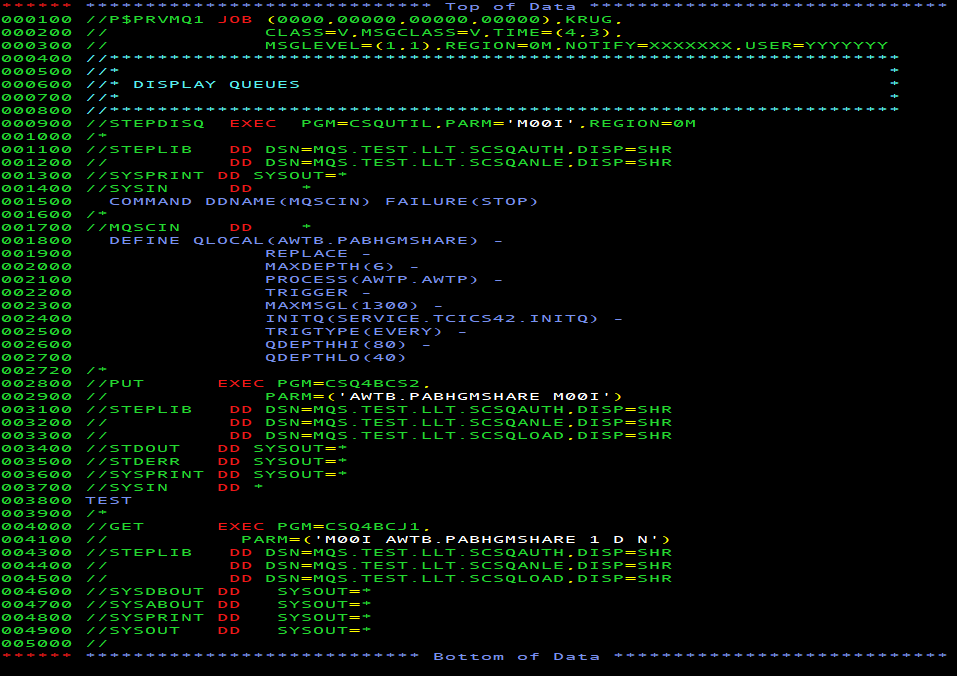
\includegraphics[width=\textwidth]{figures/defqjcl.PNG}
	\caption{Define IBM Queue, am Beispiel einer Trigger Queue}
	\label{code:defq}
\end{figure}

Ähnlich wie in Absatz \ref{sssec:db2tpl} für die Datenbank-Provisionierung beschrieben, muss der CSD Datei eine weitere Gruppe für den Queuemanager angegeben werden.
Zu sehen in Abbildung \ref{code:addCSD} in Zeile 11.
Dadurch hat eine Anwendung in dieser CICS-Instanz Zugriff auf alle Queues, die sich innerhalb dieses Managers befinden.
Des Weiteren ist die Aufnahme weiterer IBM MQ-System-Bibliotheken in der \glqq createCICS.jcl\grqq-JCL-Datei notwendig.

\section{Entwicklungsstage}
Innerhalb der Entwicklungsstage sind die Sicherheits- und Rechtevorschriften schärfer als auf dem Testplex.
So wäre es zwar möglich, alle für die administrativen Aufgaben notwendigen Rechte einer persönlichen UserID zu geben.
Dies würde aber bedeuten, dass auch alle Anwender (Entwickler) dieses Templates diese Rechte benötigen würden.
Damit bestünde eine potentielle Gefahr für das System, da sie damit auch außerhalb des Templates diese Rechte besitzen würden.
Somit wurde in Absprache mit den Administratorenteams für CICS und IBM MQ festgelegt, hierfür jeweils einen technischen User\footnote{User ID mit zunächst keinen Berechtigungen} zu beantragen.
Diesem werden nur die für das Template benötigten Rechte übergeben und er ist somit Use-Case-spezifisch.
Um als Anwender das Template nutzen zu können, werden nur die Rechte benötigt, Jobs mit diesen technischen Usern ausführen zu dürfen.
Für Db2 ist ein solcher User nicht notwendig, da es sich beim Datenbankmanagementsystem hinter der REST-API um DB0C\footnote{Siehe Absatz \ref{sssec:db2}} handelt und jeder Entwickler in dieser \glqq DB2-Sandbox\grqq{} seine Datenbanken verwalten darf. 

Bei der Übertragung des Templates vom Testplex in die Entwicklungsstage waren Anpassungen in allen drei Bereichen des Templates notwendig.

\subsection{CICS Anpassung}\label{ssec:cicsentw}
Damit der CICS spezifische technische User zum Einsatz kommt, musste der \glqq Job\grqq{} Baustein jeder JCL in jedem Step modifiziert werden.
Dafür bietet z/OSMF die Möglichkeit, beim Zuweisen des Tenants eine Standard Jobkarte\footnote{Beschrieben im Glossar Eintrag \Gls{Batch-Job}}, die vor jedem Job des Templates eingefügt wird, zu hinterlegen.
Die CICS spezifischen Dateien können von der täglichen Datensicherung der Entwicklungsstage ausgeschlossen werden, da diese bei der Deprovisionierung gelöscht werden.
Um dies zu gewährleisten, musste der Messageclass Parameter mit dem Wert  \glqq NONE\grqq{} angegeben werden.

Als Vorlage für die spezifische CSD Datei, die im Template genutzt wird, wird die Standard Entwicklunsgstage CSD genutzt.
In der Entwicklungsstage kommen im Vergleich zum Testplex andere Db2 und IBM MQ Bibliotheken zum Einsatz.
Dahingehend wurde die \glqq createCICS.jcl\grqq-JCL-Datei angepasst.
Zusätzlich musste ein SIT Parameter angepasst werden, so dass die Log Dateien in der Entwicklungsstage funktionsfähig sind.
Eine weitere CSD Gruppe für die Verkettung der Anwendungsbibliotheken musste hinzugefügt werden.
Siehe Zeile 16 im Codeabschnitt \ref{code:createGrp}.
Diese sorgt dafür, dass die Bibliotheken, die die kompilierten Programme der kompletten Entwicklungsstage beinhalten, zur Verfügung stehen. 
Dazu kam noch eine neue Bibliothek.
Diese dient später als Ablageort der kompilierten Programme, die explizit nur in dieser CICS-Instanz vorhanden sind und dort getestet werden sollen.
Diese Verkettung ist ein Standardvorgehen innerhalb der DATEV e.G., mit dem es möglich ist, neue Programmversionen und Schnittstellen zu testen und Zugriff auf notwendige, in Entwicklung bereitstehende sonstige Module zu haben.

\subsection{Db2 Anpassung}\label{ssec:db2entw}
Um die Datenbankstruktur der DATEV-Rechnungsschreibung im DB0C Datenbankmanagementsystem nachzustellen, d.h. ein isoliertes Sandbox-Datenbank-System, zu provisionieren, wurde eine genaue technische Analyse der DATEV-Rechnungs-schreibungsdatenbank durchgeführt.
Dabei stellte sich heraus, dass die Komplexität der benötigten Tabellen sehr hoch ist.
So wird auf drei Tabellen für die Ermittlung der Produktstammdaten lesend zugegriffen, auf neun weitere bei der Bestimmung der Preisabhängigkeiten.
Auf die Tabellen wird nicht direkt zugegriffen, sondern über Views\footnote{Alias einer Datenbankabfrage, auf die wie auf eine normale Tabelle zugegriffen werden kann}.
Bei den meisten werden innerhalb der View noch weitere Tabellen, teilweise aus anderen Datenbanken, gejoint.
Insgesamt besteht das System aus vierzehn Tabellen, die auf vier Datenbanken aufgeteilt sind, und zwölf Views für den Zugriff auf diese Tabellen.

Um dies in einer Db2-Sandbox-Instanz\footnote{Siehe Absatz \ref{sssec:db2}} nachzubilden, sind sog. \Gls{ddl} Skripte notwendig. 
Mit der Erstellung wurde von der Db2 Administration begonnen.
Es stellte sich heraus, dass bereits für einen kleinen Teil an Tabellen circa 600 Zeilen DDL Code\footnote{Im Anhang \ref{app:ddl} zufinden} notwendig sind.
Eine vollständige Provisionierung eines so komplexen Datenbanksystems übersteigt den zeitlichen Rahmen dieser Arbeit.
Sollte sich die Provisionierung generell als zielführend erweisen wird dieser Einmalaufwand erbracht werden.
Im weiteren Lebenszyklus der Anwendung kann auf diese Db2 jederzeit zugegriffen werden, Änderungen sind ein erheblich geringerer Aufwand als die Initialleistung.

Für die weiteren Schritte der hier vorliegenden Arbeit wurden deshalb die bereits im Datenbankmanagementsystem DB0T vorhandenen Datenbanken der DATEV-Rechnungsschreibung genutzt.
Hierfür mussten die dafür vorgesehenen Variablen in der Eingabedatei des Templates angepasst werden.
Dadurch ändert sich die Gruppe in Zeile acht im Codeabschnitt \ref{code:addCSD} von \glqq DB0C\grqq{} auf \glqq DB0T\grqq.
Außerdem wurden sowohl in der Provisionierungs- als auch in der Deprovisionierungsdatei die Datenbanksteps auskommentiert, da diese für den weiteren Test in der Entwicklungs-Stage nicht mehr zum Einsatz kommen.

\subsection{IBM MQ Anpassung}\label{ssec:mqentw}
Da für die DATEV Rechnungsschreibung, wie im Absatz \ref{ssec:preis} beschrieben, sehr viele gleichartige Queues benötigt werden, wurde für die Erstellung dieser von den IBM MQ Administratorenteam ein \Gls{rexx} Skript angefertigt.
Dies geschah unabhängig dieser Arbeit zum Zeitpunkt der Einführung des aktuellen DATEV Rechnungsschreibungsprozesses.
Dieses Skript steht dieser Arbeit zur Verfügung.
Für die Provisionierung IBM MQ Queues waren folgende Arbeitsschritte notwendig.

\begin{samepage}
\begin{itemize}
\item Anpassung des zur Verfügung stehenden Skriptes
\item Implementierung von Jobs für restliche Queues (d.h. nicht im REXX Skript enthalten)
\item Anpassung der CICS CSD Datei
\end{itemize}
\end{samepage}

Hierfür wurden zunächst die Eingabeparameter durch vorher angelegte Templatevariablen ersetzt.
Diese steuern, wie viele Queues jeweils angelegt werden, auf welchen Queue Manager die Queues angelegt werden und den ersten Qualifier des Queuenamens.
Für den restlichen Queuenamen existiert auch eine Variable, in dieser werden die Namen als Komma separierte Liste angegeben und ausgelesen.
Anhand dieser Namen wird  die maximale Queuetiefe und die maximale Länge einer einzelnen Nachricht festgelegt.
Im Original-Skript wurden die Queues mit Hilfe einer Queue, die als Vorlage dient, angelegt.
Im Fall einer Provisionierung kann nicht davon ausgegangen werden, dass diese Vorlagen zur Verfügung stehen.
Deshalb wurden die benötigten Parameter explizit manuell angegeben.
Um die damit erstellten Queues zu testen, wurde eine Routine entwickelt, die eine Nachricht auf die Queue schreibt und diese wieder abholt.
Anschließend wurde das Skript in den Provisionierungsworkflow mit Hilfe eines neuen Steps aufgenommen.

Für die Deprovisionierung der Queues besteht noch kein Skript.
Als Grundlage kann das vorher angepasste Provisionierungsskript dienen.
Hierfür musste der \glqq Define\grqq-Befehl für die Erstellung von Queues durch den \glqq Delete\grqq-Befehl ausgetauscht werden.
Die Logik für die Ermittlung der maximalen Queuetiefe und der maximalen Nachrichtenlänge wird dafür nicht mehr benötigt und konnte entfernt werden.

Die durch die beiden Skripte erstellten Queues sind im Rahmen der DATEV Rechnungssschreibung nur für den Datenaustausch zwischen der CICS Transaktion für die Preisermittlung und dem Batch Ablauf zuständig.
Wie in Absatz \ref{ssec:preis} beschrieben, benötigt der Ablauf noch weitere Queues.
Da es sich hierbei um spezielle Queues handelt, wurde auf die im Absatz \ref{sssec:mqtplx} gezeigte Technik zurückgegriffen.
Bei der Antwort-Queue für die Ermittlung der Listenpreise handelt es sich um eine Queue ohne besondere Parameter.
Es werden noch zwei Trigger-Queues benötigt, die über Processes\footnote{Siehe Absatz \ref{sssec:process}} eine Transaktion im CICS starten.
Als letzter Baustein für das Triggering der Transaktion wird noch eine Initiation Queue benötigt.
Diese muss im CICS hinterlegt sein.

Jeder CICS-Instanz kann nur eine Initiation Queue zugewiesen sein.
Dadurch benötigt jedes CICS eine eigene Initiation Queue.
Die Zuweisung geschieht in der IBM MQ CSD Gruppe.
Somit müsste für jede provisionierte CICS-Instanz eine solche CSD Gruppe angelegt werden.
In Absprache mit der IBM MQ-Administrations wurde entschieden, die Verwaltung der IBM MQ CSD Gruppe komplett im Template durchzuführen.
Diese Entscheidung hatte eine Änderung des in Abbildung \ref{code:addCSD} gezeigten Codes der \glqq InitAdditionalCSD.jcl\grqq, der durch einen Workflowdefinitionfile-Step dem Template zugeordnet ist, zur Folge.
So wird, wie in Abbildung \ref{code:createGrp} in Zeile sieben bis zehn dargestellt, zunächst eine Gruppe angelegt und anschließend wird diese Gruppe dem CSD (Zeile fünfzehn) hinzugefügt.

\begin{minipage}{\linewidth}
\lstinputlisting[caption={Erstellung einer neuen CSD Gruppe mit Hilfe eines Jobs am Beispiel des \glqq InitAdditionalCSD.jcl\grqq-Jobs },captionpos=b,label={code:createGrp}]{listings/InitAdditionalCSD.jcl}
\end{minipage}

Für jeden IBM MQ bezogenen Job wurde die Jobkarte angepasst und der technische User der CICS-Administration durch den technischen User der IBM MQ-Administration, der für administrative Aufgaben berechtigt ist, ausgetauscht.

\subsection{Testablauf}
Für die Prüfung der Funktionsfähigkeit der so generierten Laufzeitumgebung steht dieser Arbeit ein Testablauf zur Verfügung.
Dieser wurde von den Mitarbeitern der DATEV Rechnungsschreibung bereitgestellt.
Dabei handelt es sich um einen Teilablauf des gesamten DATEV Rechnungsschreibungsprozesses.
In diesem Ablauf wird nur die Preisermittlung, die die Laufzeitumgebung CICS benötigt, getestet.
Als Eingabe dienen vordefinierte Dateien mit Testdaten, die Ergebnisse werden zur Prüfung ebenfalls in Dateien geschrieben.
Der Ablauf liegt in Form von zwei Jobs vor.
Beide sind in der gleichen JCL Datei definiert, somit starten beide zeitgleich. 
Dies ist notwendig, da der erste Job die Verarbeitung im CICS über die Queues startet und der zweite auf die Ergebnisqueues lauscht.

Um den Ablauf in der provisionierten Laufzeitumgebung zu starten, musste lediglich der verwendete Queue Manager angepasst werden.
Über die Queues und das verwendete Triggering wird die Transaktion im provisionierten CICS gestartet.
Um das Ergebnis der Anwendung zu prüfen, wurde dies mit dem gleichen Testablauf und den gleichen Eingabedateien in der aktuell existierenden Testumgebung der DATEV e.G. Rechnungsschreibung durchgeführt.
Bei einem anschließenden Vergleich der Ausgabedateien beider Läufe waren keine Abweichungen festzustellen und der Test wird somit als erfolgreich bewertet.

\section{Bereitstellungsprozess aktuelles Template}\label{sec:akttemp}
Bei dem Bereistellungsprozess, der durch das aktuelle Template möglich gemacht wird, sind drei Fälle zu unterscheiden:

\begin{samepage}
\begin{enumerate}
\item Use-Case: Neue Template Instanz\\
Ein Entwickler möchte eine Programmänderung auf einer isolierten Laufzeitumgebung testen.
Dadurch wird eine neue Instanz eines Templates benötigt.
Dem Entwicklerteam steht das Template in z/OSMF zur Verfügung und es wurde noch keine Instanz dieses Templates provisioniert.

\item Use-Case: Zusätzliche Template Instanz\\
Ein weiterer Entwickler möchte parallel zu einem anderen Entwickler eine weitere Programmänderung (anderer \glqq Git-Branch\grqq) auf einer isolierten Laufzeitumgebung testen. 
Nur diese Änderung soll getestet werden, unabhängig von anderen parallelen Aktivitäten in der Anwendung. 
Dem Entwicklerteam steht dieses Template in z/OSMF zur Verfügung aber es wurde  bereits eine Instanz dieses Templates bereitgestellt. 
Um isoliert von dieser existierenden Instanz und den darin vorhandenen Änderungen zu testen, wird eine weitere Instanz benötigt.

\item Use-Case: Änderungen durch Administratorenteam\\
Die Provisionierung  einer IBM MQ Instanz soll z.B. von REXX Skripten auf eine REST-API umgestellt werden.
Dies hat Änderungen an Workflowdefinitionfiles zur Folge.
Hier ist zwischen zwei weiteren Fällen zu unterscheiden:
\begin{enumerate}
\item Das Template wurde noch nicht veröffentlicht.
\item Das Template wurde veröffentlicht.
\end{enumerate}
\end{enumerate}
\end{samepage}

\subsection{Use-Case: Neue Template Instanz}
Der Entwickler meldet sich an der z/OSMF Oberfläche an und klickt auf den Menüleistenpunkt \glqq Cloud Provisioning\grqq.
Anschließend öffnet er die \glqq Software Services\grqq{} und wählt dort das oben genannte Template aus.
Nun kann er mit einem Klick auf \glqq Run\grqq{} (Siehe Abbildung \ref{fig:runtemp}) eine neue Instanz erzeugen.
Mit dieser Instanz kann er seine Programmabläufe testen.
\begin{figure}[h]
	\centering
	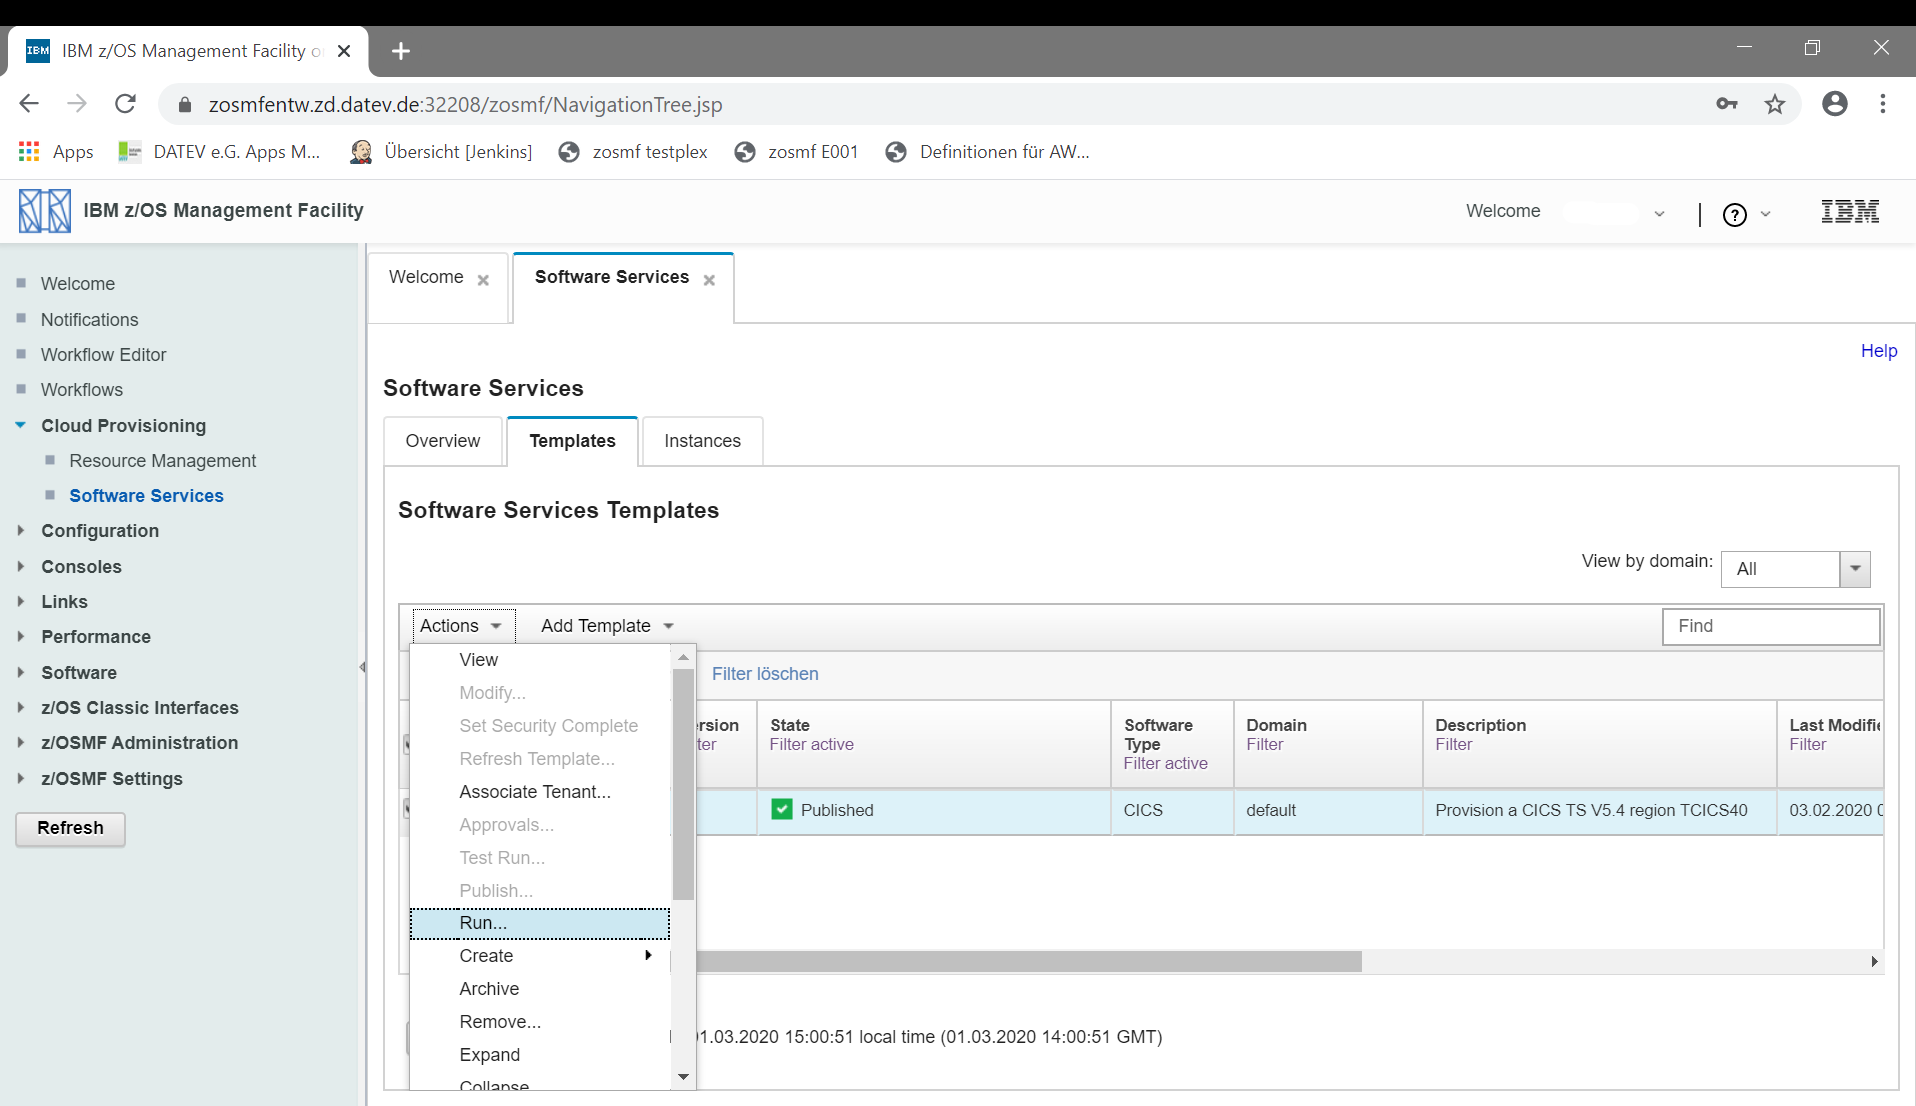
\includegraphics[width=\textwidth]{figures/published.png}
	\caption{Erzeugen einer Instanz mit dem \glqq Run\grqq-Befehl auf einem veröffentlichten Template in der z/OSMF Oberfläche}
	\label{fig:runtemp}
\end{figure}

\subsection{Use-Case: Zusätzliche Template Instanz}\label{ssec:akttemp2fall}
Mit dem aktuellen Stand des implementierten Templates muss der Entwickler wissen, an welchem Speicherort das Template abgelegt ist, da er die Template-Dateien - nicht die Workflowdateien - kopieren muss.
Es sind Änderungen am Variableinputfile notwendig.
Unter anderem ist eine andere CICS Application ID zu wählen, der Entwickler muss dafür wissen welche CICS Application ID von noch keiner Instanz genutzt wird.
Um die Queues und IBM MQ Prozesse aus Fall eins nicht zu überschreiben, muss  ein anderer Queue Manager vom Entwickler gesetzt werden.
Dieser Queue Manager muss von dem zuständigen Administratorenteam manuell bereitgestellt werden.
Die Erzeugung einer von Fall eins unabhängigen Instanz setzt die Aufnahme eines neuen Templates, welches die veränderten Dateien beinhalten, in z/OSMF voraus.
Anschließend kann wie in Abbildung \ref{fig:runtemp} dargestellt, eine weitere Instanz erzeugt werden.

\subsection{Use-Case: Änderungen durch Administratorenteam}
Ein Template ist dann veröffentlicht, wenn es den berechtigten Teams zur Verfügung steht.
Zunächst muss der Speicherort der zu bearbeitenden Workflowdefinitionfiles bekannt sein.
Anschließend kann die Änderung mit einem Editor nach Wahl durchgeführt werden.

\subsubsection{nicht veröffentlichtes Template}
Die Änderungen können vom Administratorenteam ohne Bedenken durchgeführt werden, da das Template noch keinem Entwicklerteam zur Verfügung steht.
Das diese Änderungen auch ins z/OSMF übernommen werden, muss das Template mit Hilfe der z/OSMF Oberfläche aktualisiert werden.
Dies ist per Mausklick möglich.

\subsubsection{veröffentlichtes Template}
Die Änderungen können vom Administratorenteam zwar durchgeführt werden, aber die z/OSMF Oberfläche bietet nicht mehr die Möglichkeit das Template zu aktualisieren.
So wird die Funktionsfähigkeit der veralteten Instanzen weiterhin sicherzustellen.
Es muss eine neue Version des Templates erzeugt werden.
Dies ist auch per Mausklick zu lösen.

\section{Fazit Realisierung}
Am Ende der Realisierung steht ein funktionsfähiges Template.
Dieses Template provisioniert ein für die Rechnungsschreibung individualisiertes CICS und die benötigten IBM MQ Queues. 
Wie in Absatz \ref{ssec:db2entw} beschrieben, wurde die Provisionierung einer spezifischen Db2 Datenbank wegen hoher Komplexität für diese Arbeit außen vorgelassen
Auf dem Testplex wurde bewiesen, dass die Provisionierung einer Datenbank möglich ist.
Die Provisionierung der anwendungsspezifischen Db2-Tabellen wäre mit hohem einmaligen Arbeitsaufwand ebenfalls möglich.
Ein Testablauf der Beispielanwendung DATEV-Rechnungsschreibung in einer provisionierten, isolierten CICS-Laufzeitumgebung konnte korrekt durchgeführt werden.

Folgende Probleme wurden im Rahmen der Implementierung erkannt:

\begin{samepage}
\begin{itemize}
\item Nicht sprechende Fehlermeldungen von z/OSMF
\item Nicht identifizierbare Programmiersprache
\item Nicht optimales Zugriffsrechtekonzept
\end{itemize}
\end{samepage}

Als erstes Problem sind die nichtsprechenden Fehlermeldungen von z/OSMF, Abbildung \ref{fig:zosmffehler}, zu nennen.
\begin{figure}[h]
	\centering
	
\includegraphics[width=\textwidth]{figures/zosmffehlermeldung.png}
	\caption{Beispiel einer Fehlermeldung von zOSMF}
	\label{fig:zosmffehler}
\end{figure}
Z.B. wird bei dem Hinzufügen und Aktualisieren eines Templates in z/OSMF das Template und damit alle dazu benötigten Dateien (Actiondefinitionfile, Workflowdefinitionfiles, Variableinputfile, JCL-Dateien und REXX-Skripte) auf Syntaxfehler geprüft.
Die in Abbildung \ref{fig:zosmffehler} gezeigte Meldung tritt dann ein, wenn in einer dieser Dateien ein Syntaxfehler vorhanden ist.
Beispielsweise, wenn in einer JCL-Datei das Zeichenlimit von 80 Zeichen pro Zeile überschritten wird, dafür genügt schon ein \glqq Blank\grqq.
Wie zu erkennen ist, zeigt die Fehlermeldung weder welcher Fehler genau vorliegt, noch in welcher Datei dieser auftritt.
Zudem auch keine genaue Anzahl an auftretenden Fehlern.
Dieser Umstand, kombiniert mit 36 bestehenden Dateien, erschwert die Fehlersuche.

Im Gegensatz dazu wird im Fehlerfall zur Laufzeit eines Workflow-Steps immer der Fehlercode und der genaue Ort des Fehlers ausgegeben.
Beispielsweise wird bei einem Workflow-Step, in dem ein REST Aufruf durchgeführt wird und ein Fehler auftritt, der Requestcode und die hinterlegte Fehlermeldung an der z/OSMF Oberfläche angezeigt. 

Ein weiteres Problem ist eine nicht genau identifizierbare Programmiersprache, die für die dynamische Generierung von Skripten im Worfklow genutzt wird.
Sie kommt unter anderem in den JCLs und REXX-Skripten, die dem Template über Workflowdefinitionfile-Steps zugeordnet werden, vor.
Um diese Sprache einzusetzen muss am Zeilenanfang ein \glqq\#\grqq{} angegeben werden.
Diese Sprache bietet einige Features.
So ermöglicht diese die dynamische Wertzuweisung von zum Beispiel REXX-Variablen durch Variablen des Templates.
Außerdem besteht eine Art von String Verarbeitung.
In Abbildung \ref{code:qsauslesen} ist ein Beispiel zu sehen.
Dort werden die Queuenamen, die als kommaseparierte Liste in der Templatevariable \glqq DFH\_MQ\_QUEUENAMES\grqq{} angegeben sind, ausgelesen und in eigenen REXX Variablen gespeichert.
Zu sehen ist zunächst eine \glqq set\grqq{} Anweisung, mit der Variablen zugewiesen werden können, If-Bedingungen und eine foreach-Schleife stehen außerdem zur Verfügung.

\begin{minipage}{\linewidth}
\lstinputlisting[caption={Auslesen der \glqq DFH\_MQ\_QUEUENAMES\grqq{} Variablen und schreiben in REXX Variablen (Zeile 52 bis 61 aus \glqq defineQsRexx.jcl\grqq, siehe Anhang \ref{app:qsrexx})},captionpos=b,label={code:qsauslesen}, firstline=52, lastline=62]{listings/DefineQsRexx.jcl}
\end{minipage}

In Abbildung \ref{code:qsauslesenlaufzeit} wird das Ergebnis, welches beim Run erzeugt wird, dargestellt.
Es ist zu erkennen, dass nur noch die für das REXX Skript notwendigen Codeabschnitte vorhanden sind.
Dadurch können sehr dynamische Templates erstellt werden.
Jedoch wurde weder eine Dokumentation zu dieser Sprache, noch eine Aussage, um welche Sprache es sich genau handelt gefunden.
Somit liegt dem Wissen über diese Sprache nur der Code aus Beispielen der IBM zugrunde.

\begin{minipage}{\linewidth}
\lstinputlisting[language=Rexx,caption={Zur Laufzeit erzeugtes Skript, der Grundlage aus Codeabschnitt \ref{code:qsauslesen}},captionpos=b,label={code:qsauslesenlaufzeit}]{listings/qsauslesenlaufzeit.rexx}
\end{minipage}

Ein weiterer Problempunkt ist das mit z/OSMF und dem Template einhergehende Zugriffsrechtekonzept.
Die z/OSMF Berechtigungsgruppen passen nicht zu de DATEV e.G. internen Richtlinien.
Die Aufnahme in eine solche Gruppe, um zum Beispiel die z/OSMF Oberfläche nutzen zu dürfen, geschieht auf Zuruf und manuelles Hinzufügen einer User ID durch einen Mitarbeiter, des RACF-Teams.
Generell ist der Einsatz einer für das ganze Template gültigen Standard Jobkarte, um technische User verwenden zu können, nicht optimal.
z/OSMF bietet hier eigentlich eine Möglichkeit in der Stepdefinition einen \glqq runAsUser\grqq{} anzugeben.
Unter diesem User würde der Step dann ausgeführt werden.
Folglich ist das die Stelle, an der zum Beispiel für CICS Steps der technische User für administrative CICS Aufgaben angegeben werden müsste.
Damit würde das Gewähren der expliziten Rechte zum Starten eines Jobs mit der technischen User ID entfallen und damit die manuelle Arbeit des \glqq Gewährens\grqq.
Um jedoch einen \glqq runAsUser\grqq{} in der Workflow-Stepdefinition angeben zu können, muss in der dem Template zugewiesenen Domain ein sogenannter \glqq Cloud Security Admin\grqq{} hinterlegt sein.
Dieser würde sicherstellen, dass nur die für ein Template zugelassenen User dieses Template auch provisionieren dürfen.
D.h. es kann beispielweise sichergestellt werden, dass nur DATEV-Rechnungsschreibungs-Entwickler das DATEV-Rechnungsschreibungs Template provisionieren.
In dieser Arbeit wird die mitgelieferte \glqq Default Domain\grqq{} genutzt, in dieser ist kein \glqq Cloud Security Admin\grqq{} angegeben.
Da es sich um die Standard Domain handelt, darf diese nicht geändert werden.
Somit müsste eine eigene Domain angelegt werden um einen Cloud Security Admin  hinterlegen zu können.
Dadurch, dass sich z/OSMF bei der DATEV e.G. noch in einem Untersuchungs-Stadium  befindet, wird von der Erstellung einer eigenen Domain abgesehen.
Dadurch ist es notwendig, die nicht optimale Lösung mit der Jobkarte\footnote{Siehe Absatz \ref{ssec:cicsentw}} einzusetzen.
An diesen beiden Fällen ist zu erkennen, dass das Rechtekonzept noch nicht für einen firmenweiten Einsatz bei DATEV e.G. ausgelegt ist und noch überarbeitet und angepasst werden muss.
Dies ist jedoch explizit nicht Bestandteil dieser Arbeit.


 
